\chapter*{Red-Green-Refactor}

\ifnotes

    Learning outcomes:
    
    \begin{itemize}
        \item Describe the TDD process
        \item Explain the business value of refactoring
        \item Define what refactoring is.
    \end{itemize}
    
    Before asking students to do this exercise, explain that BDD evolved from TDD. BDD is different from TDD in that it involves the whole team, but the R-G-F cycle is the same.
    
    TDD:
    \begin{enumerate}
        \item Write a failing test OR write the next micro-specification
        \item Make the test pass as quickly as possible - SHAMELESS green
        \item Refactor - improve the structure of the code WITHOUT modifying the externally observable behaviour of the code.
    \end{enumerate}
    
    Notes:
    \begin{itemize}
        \item Picking the next test to write is hard - and takes practice.
        \item It should take only a few minutes to get a test to pass - any longer and you've bitten off too much
        \item Never refactor from red. If the current failing test demands a major refactor, revert to last Green, do the refactor and then rewrite the test.
        \item How do you ensure you haven't modified the behaviour? Run the tests!
    \end{itemize}
    
\fi

\ifcontent

    \begin{framed}
       "The bitterness of poor quality remains long after the sweetness of meeting the schedule is forgotten." -- \textit{anon}
    \end{framed}    
    
    With reference to the diagram below, explain Test Driven Development (TDD) to each other.
    
    \begin{center}
    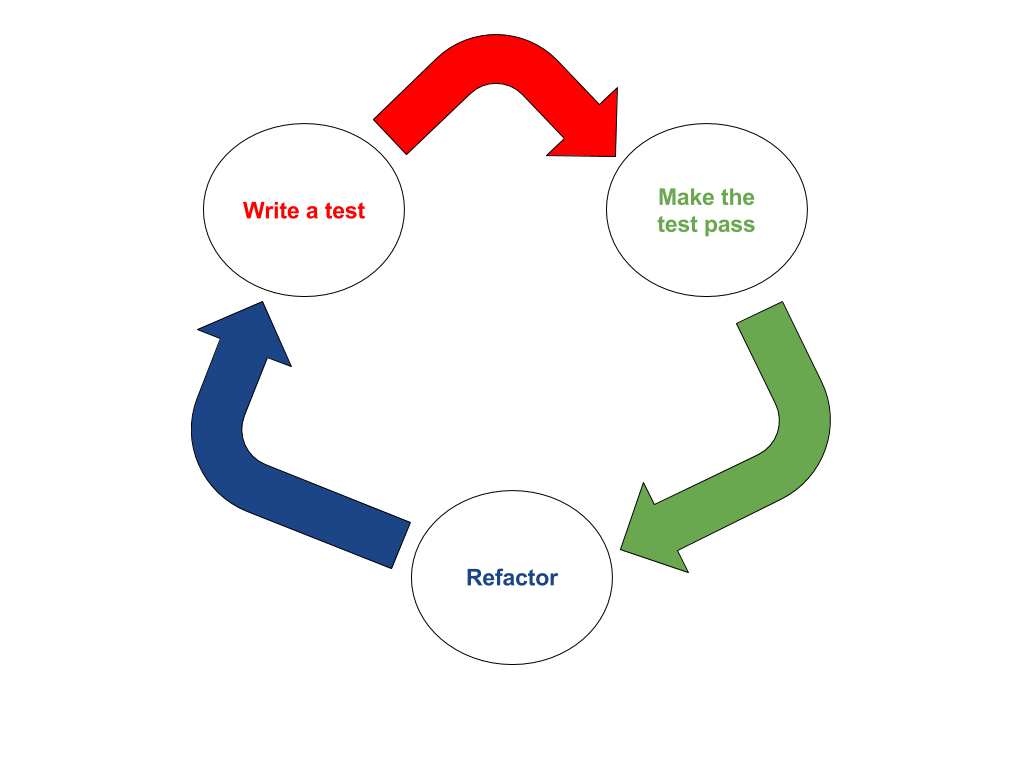
\includegraphics[width=0.8\textwidth]{images/RGR}
        
    \end{center}
    
    \QandAbox{What does "refactor" mean? Write a definition:}{1}
    
    \QandAbox{What is the business value of refactoring?}{1}
    
    \QandAbox{Should TDD stand for Test Driven Design? Why? Why not?}{1}

\fi